\documentclass[12pt,a4paper]{scrartcl}

\usepackage[english]{babel}
\usepackage[utf8]{inputenc}

\usepackage{graphicx}
\usepackage{caption}

\usepackage{latexsym,exscale,stmaryrd,amssymb,amsmath}

\usepackage[]{siunitx}
\usepackage[]{physics}

\usepackage{listings}
\usepackage{color}
\usepackage[]{datenumber}

\definecolor{dark_green}{rgb}{0,0.6,0}
\definecolor{gray}{rgb}{0.5,0.5,0.5}
\definecolor{mauve}{rgb}{0.58,0,0.82}
\definecolor{background}{rgb}{0.6,0.6,0.6}

\lstset{
  frame=single,
  backgroundcolor=\color{background},
  numberstyle=\tiny\color{gray},
  keywordstyle=\color{blue},
  commentstyle=\color{dark_green},
  stringstyle=\color{mauve},
  aboveskip=3mm,
  belowskip=3mm,
  showstringspaces=false,
  columns=flexible,
  basicstyle={\ttfamily},
  numbers=none,
  breaklines=true,
  breakatwhitespace=true,
  tabsize=4,
}

\begin{document}



\title{Advanced Computational Physics Lab - Project 3}
\maketitle

\author{Heiko Georg Menzler}
\abstract{
    In this project we look at $e^{-}e^{+} \longrightarrow q \overline{q}$ scatterings.
    The scatterings are analyzed using Monte Carlo (MC) techniques to generate scattering events.
    From the scattering events we calculate the total cross section using and comparing different optimization techniques.
    Furthermore we use at jet clustering methods for further analysis of quark-gluon showering events.
}


\vspace{20pt}
\textbf{Attention:}
Please consider that the in the repository\\ (\lstinline{github.com/h-mnzlr/acpl-particlesims.git}) included Jupyter notebooks are intended to show the thought process and present the results.
I would like to encourage you (the reader and grader) to consider them as complementary material to this report. Please go through them first. 
Effort was put into them to make them easily readable and understandable, thanks.into them to make them easily readable and understandable, thanks.

\subsection*{1a)}
In the first exercise we implement the simple MC process generation by sampling $\cos( \theta ) $ uniformly from $-1$ to $1$ and $\phi$ uniformly from $-\pi$ to $\pi$.
These scattering events we can use to calculate the total cross section as an of the differential cross section (see lecture).
See code in \lstinline{code/integrate.py} and \lstinline{notebooks/1_electron_positron.sync.ipynb}.

\subsection*{1b)}

There are two different methods of sampling the quark flavor of the generated particles to obtain to total cross section.  
In the first method the quark flavor is sampled from a random uniform distribution.
For the second method we calculate the integral for every flavor and average the results.
For now the simulations are only run with fixed beam energy $s = m_Z^2$ with $m_Z$ being the mass of the Z boson.

\begin{figure}[htpb]
    \centering
    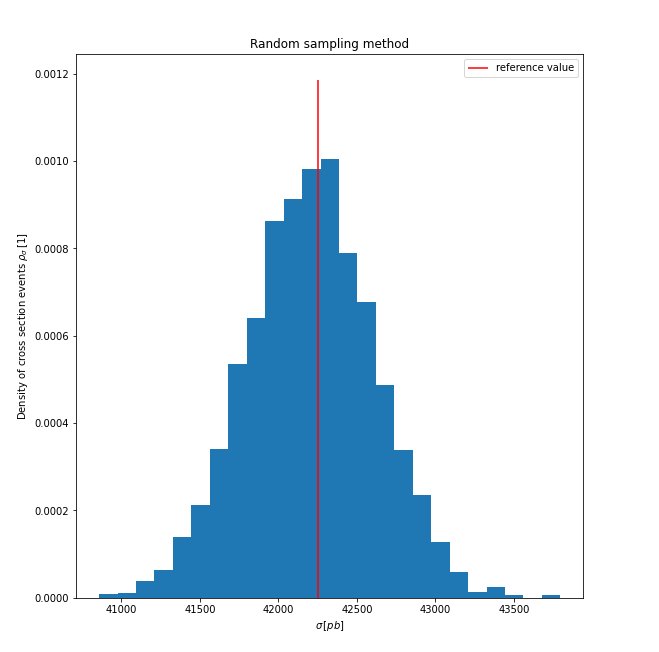
\includegraphics[width=0.4\textwidth]{figures/ex_1b_random_sampling.png}
    \caption{Density of cross section values generated over \num{1000} realizations of the MC process, sampling the quark flavors uniformly.
        The reference value of \SI{42250(50)}{\pico\barn} is marked by a red line.
    }
    \label{fig:random_sampling}
\end{figure}

\begin{figure}[htpb]
    \centering
    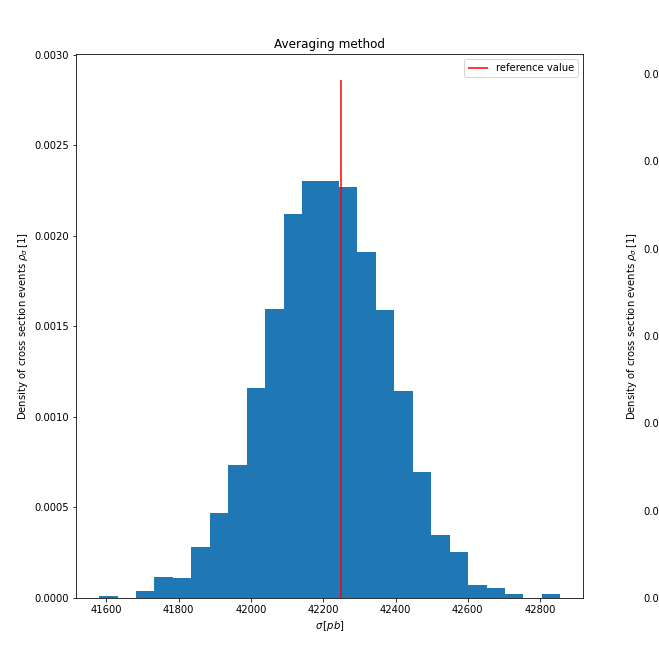
\includegraphics[width=0.4\textwidth]{figures/ex_1b_averaging_method.png}
    \caption{Density of cross section values generated over \num{1000} realizations of the MC process, averaging over the quark flavors of the possible scattering events.
        The reference value of \SI{42250(50)}{\pico\barn} is marked by a red line.
    }
    \label{fig:averaging_method}
\end{figure}    

In figures \eqref{fig:random_sampling} and \eqref{fig:averaging_method} you can see the density of total cross sections generated from the MC scattering process.
In figure \eqref{fig:random_sampling} the quark flavors were sampled uniformly and in figure \eqref{fig:averaging_method} the resulting cross section was averaged over events with all the different quark flavors.

One can see that both processes reproduce the correct mean value but they exhibit slightly different statistics.
For the random sampling method the standard deviation is around three times as large (also see the notebook), but calculating one of the realizations for the random sampling method is also around four times faster.

\begin{figure}[htpb]
    \centering
    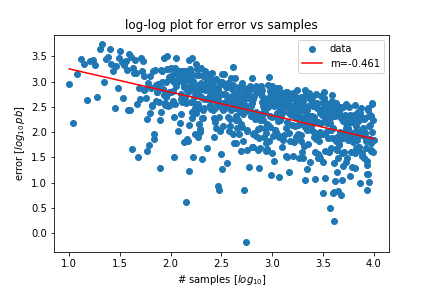
\includegraphics[width=0.8\textwidth]{figures/ex_1b_error_vs_samples_loglog.png}
    \caption{
        In this figure one can see the log-log plot of the deviation from the reference value for the total cross section $\sigma$ against the number of samples used in the MC integration.
        To show the trend of the datapoints, a linear regression has been fitted to the datapoints and the slope $m = -0.461$ has been extracted.
    }
    \label{fig:figures-ex_1b_error_vs_samples_loglog-png}
\end{figure}
        
In figure \eqref{fig:figures-ex_1b_error_vs_samples_loglog-png} we can see that there is random noise between different realization.
Still we can show from the linear regression over the whole data, that the error scales (at least very close) like $\frac{1}{\sqrt{N} }$ as expected from the theory of MC simulations (lecture).



\section*{1c)}

Now we also want to sample the energy of the incoming particle beam s.t. $s$ is uniformly distributed between $(m_Z - 3 \Gamma_Z)^2$ and $(m_Z + 3 \Gamma_Z)^2$. $\Gamma_Z$ is the decay width of the Z boson.

\begin{figure}[htpb]
    \centering
    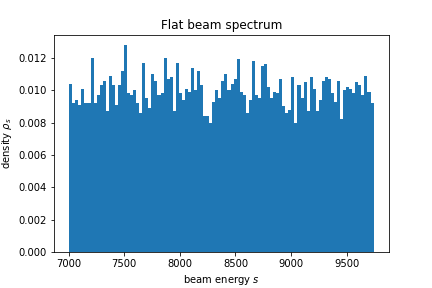
\includegraphics[width=0.8\textwidth]{figures/ex_1c_histogram_s.png}
    \caption{}
    \label{fig:histogram_s}
\end{figure}

In figure \eqref{fig:histogram_s} one can see one particular sampling of the flat beam spectrum of uniformly sampled $s$ for \num{1000} samples.
Find the code for the sampling in \lstinline{code/integrate.py}.


\section*{1d)}

\begin{figure}[htpb]
    \centering
    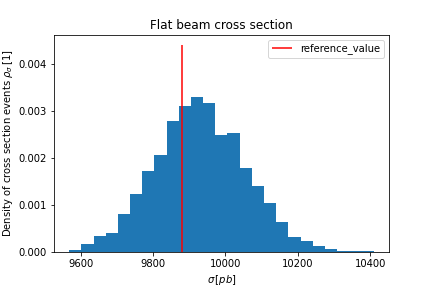
\includegraphics[width=0.8\textwidth]{figures/ex_1c_flat_beam_hist.png}
    \caption{
        Density of cross section values generated over \num{1000} realizations of the MC process, sampling the quark flavors uniformly and the beam energy from $(m_Z - 3 \Gamma_Z)^2$ to $(m_Z + 3 \Gamma_Z)^2$.
        The reference value of \SI{9880(50)}{\pico\barn} is marked by a red line.
    }
    \label{fig:figures-ex_1c_err}
\end{figure}

In figure \eqref{fig:figures-ex_1c_error_vs_samples_loglog-png} one can see the statistics of the MC integration process.
Again we can confirm that the MC process reproduces the reference value in the given error intervals.

\begin{figure}[htpb]
    \centering
    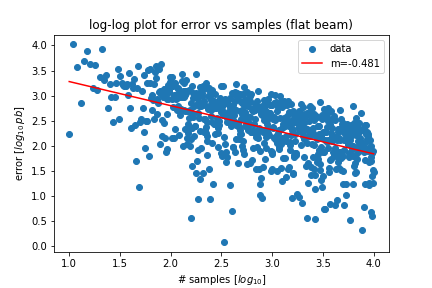
\includegraphics[width=0.8\textwidth]{figures/ex_1c_error_vs_samples_loglog.png}
    \caption{
        In this figure one can see the log-log plot of the deviation from the reference value for the total cross section $\sigma$ against the number of samples used in the MC integration for the flat beam spectrum.
        To show the trend of the datapoints, a linear regression has been fitted to the datapoints and the slope $m = -0.461$ has been extracted.
    }
    \label{fig:figures-ex_1c_error_vs_samples_loglog-png}
\end{figure}

Similarly as in b) we have created the log-log plot for the deviation of the MC simulation from the reference value.
Furthermore we can again confirm that the error scales like $\frac{1}{\sqrt{N} }$ with the number of samples $N$.

We have seen that the values for the total cross section are a lot smaller than those generated at a fixed $s$.
This is largely due to the fact that the differential cross section has a maximum at $s = M_Z^2$.
Therefore sampling around the maximum will generally reduce the value of whole integrated space when averaging.

% TODO: finish 1d

\section*{1e)}

Using the \lstinline{vegas} python package we can use state-of-the-art optimization techniques for our MC simulations.
In figure \eqref{fig:figures-ex_1e_grids-png} one can see the summary output of the VEGAS integration over 10 iterations.
We can see that the integration becomes more accurate for every iteration.

This is due to -- as we can also see in the second graphic of figure \eqref{fig:figures-ex_1e_grids-png} -- the adaptive algorithm sampling certain parts of the integration interval more dense than others.
Specifically, the region around the peak of the spectrum at $s = M_Z^2$ is sampled a lot more densely than other parts of the distribution.

\begin{figure}[htpb]
    \centering
    
\includegraphics[width=0.8\textwidth]{figures/ex_1e_grids.png}
    \caption{Summary output of the \lstinline{vegas} package for the MC simulation and grid for the sampling in the $s$-$\cos( \theta  ) $-plane.}
    \label{fig:figures-ex_1e_grids-png}
\end{figure}

\section*{1f)}
Using the information we found in the last exercise we want to try to implement our own importance sampling algorithm.
We do so by using the mapping from the lecture, which maps uniformly sampled values to a Breit-Wiegner distribution.

First we need to obtain our new upper and lower bounds for the uniform distribution from 
\[
    \rho_{ \text{min/max} } = \arctan( \frac{(s_{ \text{min/max} - M_Z^2) } }{M_Z \Gamma_Z} ) 
.\] 

From now we can use the transformation introduced in the lecture to generate $s$ values in a Breit-Wiegner distribution.
For code see \lstinline{code/integrate.py}.

\section*{1g)}



\section*{2a)}
In exercise two we take into account that the created quarks can emit further particles, resulting in a shower of quarks and gluons.
As the coupling strength of Z boson depends critically on the energy scale we need a way to calculate this interaction strength.
The \lstinline{utils} library provided to use for the project implements such a calculator in the \lstinline{AlphaS} class.
We use it to calculate the coupling strength $\alpha(M_Z)$  as a function of the beam scattering energy $s$.

 \begin{figure}[htpb]
    \centering
    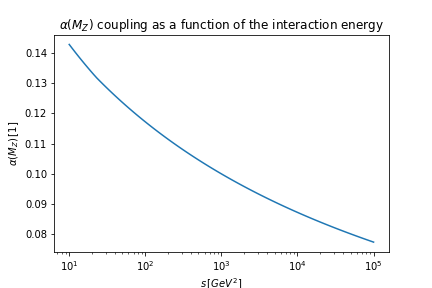
\includegraphics[width=0.8\textwidth]{figures/ex_2a_alpha_coupling.png}
    \caption{In this figure you can read of the strength of the $\alpha(M_Z)$ coupling for different scattering energies $s$.}
    \label{fig:figures-ex_2a_alpha_coupling-png}
\end{figure}

In figure \eqref{fig:figures-ex_2a_alpha_coupling-png} you can see that the coupling strength increases at low energies.
This means that when we assume $\alpha \ll 1$ we can only deal with high energy scattering processes.

\section*{2b)}
To simulate the showering process we can use the provided class \lstinline{Shower} from the \lstinline{utils} library.
Please refer to the notebook \lstinline{notebooks/2_electron_positron.sync.ipynb} for how the MC process was extended to generate events in the required format.


\section*{2c)}
We can easily transform the process from 2b) into an event Generator (python Generator) that creates events, which we can consume.
Using this procedure and the \lstinline{Shower} class we can look at how many particles are created on average.

\begin{figure}[htpb]
    \centering
    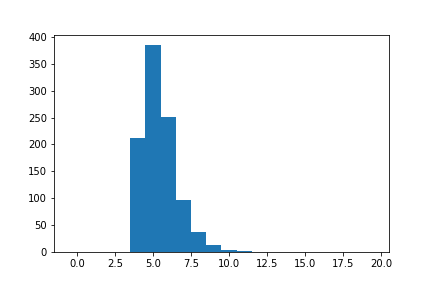
\includegraphics[width=0.8\textwidth]{figures/ex_2c_num_of_particles.png}
    \caption{Histogram of newly created particles during the shower for a total of 1000 realizations.}
    \label{fig:figures-ex_2c_num_of_particles-png}
\end{figure}

From the 1000 realizations shown in figure \eqref{fig:figures-ex_2c_num_of_particles-png} one can not only find that the average of created particles is around \num{5.541} but also that the distribution is most-likely poisson-like.
Comparing this number with the reference value of \SI{5.2(2)}{} we are slightly outside of the 1-$\sigma$ interval.


\section*{2d)}
Please refer to the code in \lstinline{code/utils/analysis.py}.

\vspace{20pt}

\emph{
    Unfortunately there are still issues in the implementation of the routine.
    Although I think I have implemented the algorithm correctly I am not sure about the implementation details required by the classes and I was unable to debug and resolve the problems in the given time frame.
}

\section*{2e)}


\begin{figure}[htpb]
    \centering
    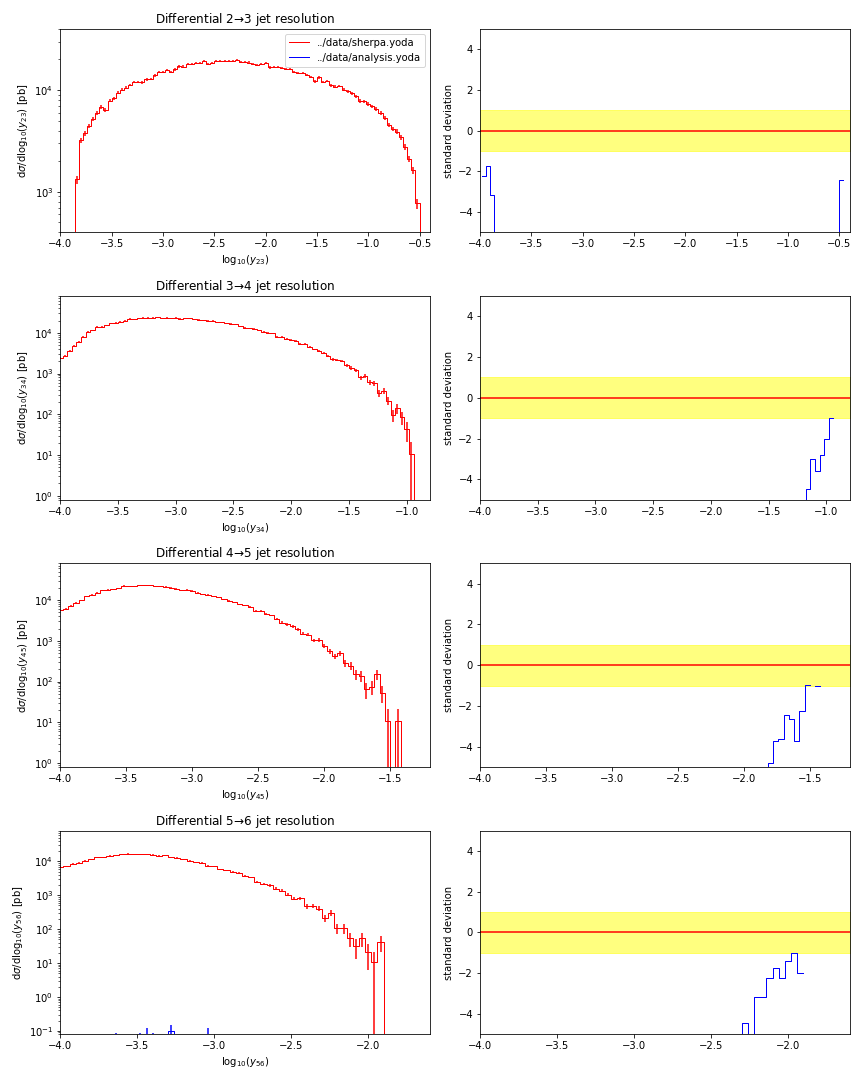
\includegraphics[width=0.8\textwidth]{figures/ex_2e_jet_histograms.png}
    \label{fig:figures-ex_2e_jet_histograms-png}
\end{figure}

Using the provided library we plot the differential jet rates against the distance between two particles (see figures in \eqref{fig:figures-ex_2e_jet_histograms-png}).

\vspace{20pt}

\emph{
    Looking at the Histogram .yoda files it looks like the events are actually being binned correctly but the histograms of the provided SHERPA
    do not line up at all, unfortunately.
}




\end{document}
